\documentclass[12pt,letterpaper]{article}

% Packages
\usepackage[margin=1in,headheight=22pt]{geometry}
\usepackage{graphicx}
\usepackage{booktabs}
\usepackage{longtable}
\usepackage{array}
\usepackage{multirow}
\usepackage{xcolor}
\usepackage{hyperref}
\usepackage[T1]{fontenc}
\usepackage[utf8]{inputenc}
\usepackage{setspace}
\usepackage{titlesec}
\usepackage{fancyhdr}
\usepackage{caption}
\usepackage{footnote}
\usepackage{enumitem}
\usepackage{amsmath}
\usepackage{float}
\usepackage{ragged2e}
\usepackage{parskip}
\usepackage{colortbl}
\usepackage{makecell}
\usepackage{tabularx}
\usepackage{lscape}
\usepackage{palatino}
\usepackage[round,authoryear]{natbib}
\usepackage{draftwatermark}
\setcounter{tocdepth}{3}
\setcounter{secnumdepth}{2}

% Colors
\definecolor{cmfmaroon}{RGB}{128,0,32}
\definecolor{cmfgray}{RGB}{90,90,90}
\definecolor{cmflightgray}{RGB}{240,240,240}
\definecolor{cmfheadergray}{RGB}{60,60,60}

\usepackage{pgfplots}
\pgfplotsset{compat=1.18}
\pgfplotsset{
    cmfaxis/.style={
        width=0.88\textwidth, height=0.46\textwidth,
        axis lines=left,
        axis line style={cmfgray, line width=0.5pt},
        tick style={cmfgray, line width=0.5pt},
        label style={font=\small, color=cmfheadergray},
        tick label style={font=\footnotesize, color=cmfheadergray},
        legend style={font=\footnotesize, draw=none, fill=none,
                      cells={anchor=west}},
        grid=major, grid style={cmflightgray, line width=0.4pt},
        enlarge x limits=0.04, scaled y ticks=false,
        x tick label style={/pgf/number format/1000 sep={}},
        y tick label style={/pgf/number format/fixed},
    },
}

\hypersetup{
    colorlinks=true,
    linkcolor=cmfmaroon,
    urlcolor=cmfmaroon,
    citecolor=cmfmaroon,
}

% ============================================================
% DRAFT CONTROLS
% Set \draftfalse before the client copy. Everything below switches off:
%   - the DRAFT watermark on every page
%   - "DRAFT" in the running header and footer, and the title-page banner
%   - red \TODO, \PEND, \NEEDSRC markers, and figure/table placeholders
%     (placeholders are boxes only while the file is missing)
% \TODO{}    = section still to write
% \PEND{}    = number awaiting a computation
% \NEEDSRC   = claim whose citation must be replaced with a primary source
% ============================================================
\newif\ifdraft
\drafttrue
\newcommand{\TODO}[1]{\ifdraft\textcolor{red}{\textbf{[TODO: #1]}}\fi}
\newcommand{\PEND}[1]{\ifdraft\textcolor{red}{[#1]}\else\textbf{??}\fi}
\newcommand{\NEEDSRC}{\ifdraft\textsuperscript{\textcolor{red}{[src]}}\fi}

\ifdraft
  \SetWatermarkText{DRAFT}
  \SetWatermarkScale{1.1}
  \SetWatermarkColor[gray]{0.88}
\else
  \SetWatermarkText{}
\fi

% FIGURE SLOT ---------------------------------------------------------
% Usage: \figslot{file-stem}{caption}{label}{what the figure should show}
% Upload the finished figure to Overleaf as figures/<file-stem>.pdf (or .png).
% Until then a red placeholder box shows the exact file name expected.
% Once the file exists the figure appears automatically. No other edit needed.
\newcommand{\figslot}[4]{%
  \begin{figure}[H]
  \centering
  \IfFileExists{figures/#1.pdf}{\includegraphics[width=0.92\textwidth]{figures/#1.pdf}}{%
  \IfFileExists{figures/#1.png}{\includegraphics[width=0.92\textwidth]{figures/#1.png}}{%
  \fcolorbox{red}{white}{\parbox[c][2.3in][c]{0.86\textwidth}{\centering
    \textcolor{red}{\textbf{FIGURE PLACEHOLDER}}\\[6pt]
    Upload as \texttt{\detokenize{figures/#1.pdf}}\\[6pt]
    \footnotesize\textcolor{cmfheadergray}{#4}}}}}
  \caption{#2}
  \label{#3}
  \end{figure}}

% TABLE SLOT (for tables not yet built) ------------------------------
\newcommand{\tabslot}[2]{%
  \begin{center}
  \fcolorbox{red}{white}{\parbox{0.86\textwidth}{\centering
    \textcolor{red}{\textbf{TABLE PLACEHOLDER: #1}}\\[4pt]
    \footnotesize\textcolor{cmfheadergray}{#2}}}
  \end{center}}

\titleformat{\section}{\large\bfseries\color{cmfmaroon}}{\thesection}{0.6em}{}[\vspace{2pt}\hrule\vspace{4pt}]
\titleformat{\subsection}{\normalsize\bfseries\color{cmfheadergray}}{\thesubsection}{0.6em}{}
\titleformat{\subsubsection}{\normalsize\itshape\color{cmfheadergray}}{}{0em}{}

\titlespacing*{\section}{0pt}{18pt}{6pt}
\titlespacing*{\subsection}{0pt}{12pt}{4pt}
\titlespacing*{\subsubsection}{0pt}{8pt}{2pt}

\pagestyle{fancy}
\fancyhf{}
\fancyhead[L]{\small\color{cmfgray}\textit{What Would a Head Tax Mean for Chicago?}}
\fancyhead[R]{\small\color{cmfgray}\ifdraft\textcolor{red}{\textbf{DRAFT}} \textperiodcentered\ \fi Center for Municipal Finance}
\fancyfoot[C]{\small\ifdraft\textcolor{red}{Working draft, not for citation or distribution} \textperiodcentered\ \fi\thepage}
\renewcommand{\headrulewidth}{0.4pt}
\renewcommand{\headrule}{\hbox to\headwidth{\color{cmfmaroon}\leaders\hrule height \headrulewidth\hfill}}

\captionsetup{font=small, labelfont=bf, labelsep=period}

\newcolumntype{L}[1]{>{\RaggedRight\arraybackslash}p{#1}}
\newcolumntype{C}[1]{>{\Centering\arraybackslash}p{#1}}
\newcolumntype{R}[1]{>{\RaggedLeft\arraybackslash}p{#1}}
\newcolumntype{Z}{>{\Centering\arraybackslash}p{0.95in}}
\newcolumntype{Q}{>{\RaggedLeft\arraybackslash}p{0.95in}}

\setlength{\parskip}{6pt}
\setlength{\parindent}{0pt}

\begin{document}

\thispagestyle{empty}
\begin{center}
    \ifdraft{\Large\bfseries\color{red} DRAFT \textperiodcentered\ NOT FINAL}\\[0.15in]\fi
    \includegraphics[width=4.5in]{logo.pdf}\\[0.5in]
    \hrule height 1.5pt
    \vspace{12pt}
    {\huge\bfseries\color{cmfmaroon} What Would a Head Tax \\[4pt] Mean for Chicago?}\\[12pt]
    \hrule height 0.8pt
    \vspace{24pt}
    {\large\color{cmfgray} Taha Rashid \\ Justin Marlowe \\[0.3in]
    Center for Municipal Finance \\
    Harris School of Public Policy\\
    University of Chicago}\\[0.4in]
    {\Large\color{cmfgray} Report \#26-04}\\[0.2in]

    {\large\color{cmfgray} \ifdraft Working draft of \fi September 29, 2026}
\end{center}

\vfill

{\scriptsize\color{cmfgray} This report was prepared by the Center for Municipal Finance at the University of Chicago, at the request of the Civic Committee of the Commercial Club of Chicago. Taha Rashid is a recent graduate of the Harris School's Master of Public Policy program. Justin Marlowe is a Research Professor and Director of the Center for Municipal Finance at the University of Chicago. For questions or comments, contact Justin Marlowe (jmarlowe@uchicago.edu). The views reported herein are those of the authors, and do not represent an official position of the University of Chicago, the Harris School of Public Policy, or the Commercial Club of Chicago. \ifdraft\textcolor{red}{\textbf{This is a working draft. Figures, estimates and text are subject to change and should not be cited or circulated.}}\fi}

\newpage

\thispagestyle{fancy}
\section*{Executive Summary}

\TODO{Draft written from current results. Trim to two pages, remove any figure that changes, and finalize last once Sections 4 and 5 are frozen. No citations in this section.}

Chicago's employer head tax was repealed in 2013, and proposals to bring it back have appeared in every recent budget cycle. The debate has mostly asked whether the tax destroys jobs. This report asks a different question: how much would the tax raise, and would employers respond to it in ways that shrink what it raises? Four findings follow.

\begin{enumerate}[leftmargin=*]
\item \textbf{The historical tax was too small to test.} The old tax cost about \$48 per employee per year, so crossing the 50-employee threshold cost a firm about \$2,400 a year. We find clustering of employers just below the threshold, but it is not attributable to the tax. It is no lower after the tax was repealed, it appears in two comparison areas that were never taxed, and it rises while the tax rate and threshold were unchanged. The proposed tax is different in kind: \$396 per employee per year with a 500-employee threshold means one hire would cost a firm about \$198,000.

\item \textbf{The historical record cannot tell us how firms would respond today.} We found no detectable avoidance at the old threshold, but the test could only have detected a large response, and we have no case in the data where the method is known to detect avoidance. The historical test also observes only single-location businesses, while about three quarters of the firms above 500 employees are multi-site.

\item \textbf{Our estimates bracket the Administration's \$82 million, and the Administration sits near the bottom of the range.} Measuring employers by their Chicago headcount, 243 firms with 388,336 employees would be above a 500-employee threshold on our central base, after removing government and a set of records with impossible headcounts. After adjusting for remote work using public Census data, revenue on that base runs from about \$81 million to about \$141 million a year, depending on which employers are exempted and on whether the tax covers all employees or only full-time employees. Across every base and adjustment we tested, it runs from about \$55 million to about \$148 million.

\item \textbf{A static base is the wrong assumption.} Any revenue projection applies the rate to a base measured before the tax exists. A large notch gives the largest and most sophisticated employers a strong reason to restructure. On our central estimates that apply the tax to all employees, erosion of the base by 21 to 42 percent would bring revenue down to \$82 million.
\end{enumerate}

What this analysis cannot settle is how much erosion would actually occur. History offers no test of a tax of this size, and no peer-reviewed causal study of a U.S. municipal per-employee tax exists.

\newpage

\tableofcontents
\newpage

%% ============================================================
\section{Introduction}
%% ============================================================

Chicago levied a tax on employers, known as the head tax, from 1974 until the end of 2013. Proposals to revive it have appeared in every recent budget cycle. The most recent, in the Mayor's 2026 budget, was left out of the budget the City Council passed in December 2025, and a new proposal is expected this fall. The debate around these proposals has settled into a familiar shape. Opponents describe the tax as a job killer. Supporters describe it as a modest levy on large employers that raised roughly \$25 million a year without observable harm. Both claims have been made repeatedly and neither has been tested carefully against data.

This report has three purposes, corresponding to the three parts of the study. The first is to establish what the research literature can and cannot say about the economic effects of employer head taxes. The second is to evaluate the revenue estimates attached to Chicago's current proposals. The third is to measure what happened in Chicago while the tax was in force.

The report's central argument is that the debate has been framed around the wrong question. Whether a head tax destroys jobs is an empirical question, and the available evidence does not support a strong affirmative answer. The more consequential question is whether the tax collects what it is projected to collect. A head tax with a size threshold gives firms near that threshold a sharp incentive to restructure so that the threshold does not bind. If firms respond, employment need not fall at all, and yet the base can erode substantially, leaving the revenue forecast wrong and the burden concentrated on employers least able to reorganize.

Answering that question requires knowing who would actually be liable, and this is where public data run into a problem. Chicago's ordinance taxed \textit{employers} according to the number of employees performing services within the city. Every public data source, however, reports \textit{establishments}: individual worksites. A firm with four Chicago offices of two hundred employees each was liable under the ordinance but appears in federal statistics as four mid-sized establishments, none of them near any threshold.

The contribution of this report is to close that gap. Using establishment-level business microdata that carries a corporate parent identifier, we filter to Chicago and then aggregate to the firm, producing a distribution of employer size measured the way the ordinance measured it. We then use the full 1997 to 2025 panel of the same data to test whether employers ever responded to the historical threshold.

Our findings are summarized in the Executive Summary and developed in Sections 4 and 5. In brief, we find no detectable avoidance of the historical threshold, and we explain why that null gives little guidance about a tax more than a hundred times larger at the threshold. We measure the base of employers a 500-employee threshold would reach, using each firm's Chicago headcount, and find that our revenue estimates bracket the Administration's \$82 million, with that figure near the bottom of the range. And we explain why any revenue projection built on a static base is fragile, since a notch of this size gives large employers a strong reason to restructure.

%% ============================================================
\section{Background and Current Policy Context}
%% ============================================================

\subsection{Chicago's Head Tax}

The City of Chicago imposed an Employer's Expense Tax, commonly called the head tax, beginning in 1974.\NEEDSRC{} The original rate was \$3 per month for each full-time employee, applying to employers with 15 or more workers in Chicago. It raised \$30.2 million in its first full year and was upheld by the Illinois Supreme Court that same year.

The rate and threshold moved several times over the following two decades. The rate fell to \$2 per employee per month in 1982, rose to \$5 in 1984, and was reduced to \$4 in 1995. The 1995 amendment also made two changes that matter for everything in this report: it raised the employee threshold from 15 to 50, and it limited the tax to full-time employees working at least half of their time within the city limits.

Table~\ref{tab:rate-history} summarizes the history. Several mayors, including Jane Byrne, Harold Washington and Richard M. Daley, stated an intention to repeal the tax but did not do so. In its final full year of operation, 2011, it raised \$23.5 million.

\begin{table}[H]
\centering
\caption{Chicago Employer's Expense Tax, rate and threshold history}
\label{tab:rate-history}
\small
\begin{tabular}{@{}llL{2.9in}@{}}
\toprule
\textbf{Year} & \textbf{Rate} & \textbf{Threshold and scope} \\
\midrule
1974 & \$3 / employee / month & 15 or more full-time employees \\
1982 & \$2 / employee / month & Unchanged \\
1984 & \$5 / employee / month & Unchanged \\
1995 & \$4 / employee / month & Raised to 50 employees; limited to full-time employees working at least 50 percent of time in Chicago \\
2012 & \$2 / employee / month & Phase-out begins \\
2014 & Repealed & Fully eliminated 31 December 2013 \\
\bottomrule
\end{tabular}
\end{table}

Two contemporaneous estimates give a sense of the tax's reach. The Chicagoland Chamber of Commerce reported that roughly 2,600 businesses and 500,000 jobs were affected in 1999. A 2011 press release from Mayor Emanuel's office stated that approximately 2,700 Chicago companies registered and paid the tax in 2009 and 2010.\NEEDSRC{}

\subsubsection{Who Was Liable: The Employer, Not the Worksite}

The unit on which the threshold was calculated is the single most consequential institutional detail in this report, and it is worth establishing carefully because both the revenue analysis in Section 5 and the empirical work in Section 4 depend on it.

Section 3-20-030(A) of the Municipal Code, effective 1 July 1995, imposed the tax on every employer who, in connection with the employer's business, engaged, hired, employed or contracted with 50 or more individuals as commission merchants and full-time employees, or any combination of the two, to perform work or render services in whole or in part within the city of Chicago. The threshold is therefore 50 \textit{or more}: an employer with 49 qualifying employees owed nothing, and an employer with 50 owed the tax on all 50.

Two further features follow directly from that language. First, the taxed unit is the employer, defined by the ordinance as any person employing one or more employees performing services within Chicago, where a person includes a corporation. It is not the worksite. Second, the count is of Chicago employees only. National headcount is irrelevant to liability, which distinguishes Chicago's ordinance from the firm-size measures available in most federal data.

The Department of Revenue's own guidance confirms the first point. A 1997 information bulletin addressed multi-location employers directly, with a worked example: a company with 60 employees distributed across three Chicago offices files a single return covering all 60, because the company controls payment of their wages.

The Department went further in 2005. Employer's Expense Tax Ruling No.~2, effective 15 September 2005, provided that for the purpose of calculating the 50-employee threshold, employees would be combined where they were employed by members of a single unitary business group. The ruling defined such a group as persons related through common ownership or control, operating in the same general line of business, and functionally integrated through centralized management over matters such as purchasing, financing, personnel and marketing. Common ownership in the case of corporations meant direct or indirect control of more than 50 percent of outstanding voting stock. The ruling described itself as a clarification of existing law rather than a change.

That interpretation was contested and upheld. In \textit{DTCT, Inc.\ v.\ City of Chicago Department of Revenue}, the Department had assessed several groups of separately incorporated McDonald's franchises, each individually below the threshold but commonly owned and centrally managed. The First District affirmed the assessments, reasoning that the ordinance's broad definition of business, which reaches entities that are subsidiary or independent, supported combining them, and that the contrary reading would allow large employers to avoid the tax by creating subsidiaries \citep{dtct2011}. Presiding Justice Garcia dissented, arguing that the Department had expanded the definition of employer without authorization from the City Council.

Two implications carry forward. The correct unit of analysis is the firm, measured by its Chicago employment. And the 2005 ruling represents a tightening of threshold enforcement \textit{within} the tax era, a second source of policy variation distinct from the 2013 repeal.

\subsection{Repealing the Head Tax}

The tax was phased out in two steps. In November 2011 the City Council approved a reduction from \$4 to \$2 per employee per month effective in 2012, and full elimination effective 31 December 2013.

The stated rationale was competitiveness: the tax was described as a penalty on hiring, and its removal as a signal to employers considering Chicago. The counterargument, then and now, is that the tax was small relative to the cost of employment and that the revenue it produced funded services with their own economic value. As Table~\ref{tab:rate-history} shows, the tax at its final rate amounted to \$48 per employee per year.

An analysis by WBEZ using city tax records obtained through a Freedom of Information Act request found that Chicago employment did rise after the repeal, but that the increase began during the recovery from the 2008 recession, before the phase-out, and was mirrored in the suburbs, which were never subject to the tax \citep{woelfel2025}. That pattern is not consistent with the repeal having caused the improvement.

\subsection{Recent Proposals}

The proposal in the Mayor's 2026 budget went through several versions: \$21 per employee per month on employers with 100 or more employees, then \$21 on 200 or more, and finally \$33 per month, or \$396 per year, on employers with more than 500 employees.\NEEDSRC{} Sources disagree on whether the threshold was ``more than 500'' or ``500 or more,'' so we report both where the difference matters. The Administration stated that the tax would apply to roughly 175 companies and would raise approximately \$82 million, a figure that implies about 207,000 covered employees. The Administration never released the list of affected companies or an exemption schedule, and a senior policy official has said the projection relied on data that were more than a decade old.\NEEDSRC{}

The City Council passed the 2026 budget 30 to 18 on 20 December 2025 without the head tax, and the Mayor declined to veto it on 23 December.\NEEDSRC{} This report therefore addresses a counterfactual that is likely to return, not a live bill.

The Administration's figures can be checked against history. At \$396 per employee per year, \$82 million implies roughly 207,000 covered employees. That is close to the WBEZ finding that, of the approximately 2,200 companies paying the head tax annually between 2000 and 2013, an average of about 188 employed 500 or more people, accounting for roughly 225,000 jobs each year, or about 21 percent of Chicago employment \citep{woelfel2025}. The correspondence is a consistency check, not independent confirmation, since the Administration's projection is reported to rest on the same historical collections.

Section 5 examines whether that base is still the right one. Two changes since 2013 pull in opposite directions: the growth of remote and hybrid work reduces the share of employees performing services within the city, while the composition and size distribution of Chicago employers has continued to shift.

\subsubsection{Head Taxes in Other Jurisdictions}

Two comparisons recur in the policy discussion.

Seattle enacted an employer head tax in May 2018, scheduled to take effect on 1 January 2019. It was repealed roughly one month after passage, following a campaign by Amazon and other Seattle employers who had pledged to place a repeal referendum on the ballot.\NEEDSRC{}

Denver has levied an Occupational Privilege Tax since 1969. It has two components, one on employees and one on employers, currently \$5.75 and \$4.00 per month respectively, rates set in 1988. The employee component applies above a monthly earnings floor. The tax is projected to generate approximately \$57 million in fiscal year 2026.\NEEDSRC{} Denver's experience is the longest continuous record of a municipal head tax in a large American city, though the low rate limits how much can be inferred about behavioral response.

%% ============================================================
\section{Insights from the Academic Literature}
%% ============================================================

\subsection{Employment and Wage Effects of Employer Head Taxes}

Direct evidence on municipal head taxes is thin. We found no peer-reviewed causal evaluation of any U.S. municipal per-employee employer tax. That is a gap this report cannot fill from the literature, and it is the reason the following subsection, on size-contingent rules, carries most of the analytical weight.

\TODO{Thematic synthesis of the remaining evidence (incidence of payroll and per-employee levies, local business tax studies, WBEZ and other descriptive work). Insert the six literature comparison tables here as they are finalized. Coordinate with Marlowe's literature refresh.}

\tabslot{Literature comparison tables (six)}{Paste the six comparison tables from the earlier Overleaf version here, or upload them as tables/lit\_tables.tex and \textbackslash input them.}

\subsection{Size-Contingent Rules and Threshold Avoidance}

The economics of a head tax with a size threshold is not primarily about the level of the tax. It is about the shape of the schedule at the threshold.

Chicago's tax created what the public finance literature calls a \textit{notch}: a point at which a small change in behavior produces a discrete jump in tax liability. Under the post-1995 ordinance, an employer with 49 qualifying employees owed nothing. An employer with 50 owed the tax on all 50, or \$2,400 a year. Hiring the fiftieth employee therefore did not cost \$48 in tax. It cost \$2,400, because that hire pulled the other 49 into liability (Figure~\ref{fig:notch}).

This is distinct from a \textit{kink}, the more common design, in which a higher rate applies only to the marginal unit above the threshold. Under a kink, the fiftieth hire would have cost \$48. The distinction matters because notches generate far sharper incentives to locate just below the cutoff, and because they create a region just above the threshold in which a firm would be strictly better off with fewer employees and more after-tax income. \citet{kleven2013} call this the dominated region, and observe that it would contain no firms at all in a world without adjustment frictions.

Their framework is the standard reference for estimating behavioral response at notches. Notches produce excess mass below the cutoff and missing mass above it, and by combining the observed bunching, which is attenuated by frictions, with the mass remaining in the dominated region, which measures those frictions, one can recover the elasticity that would govern behavior in their absence. Applied to income tax notches in Pakistan, the framework yields a result directly relevant here: observed bunching was large, frictions were also large, and the underlying structural elasticity was nevertheless modest. Their conclusion is that notches are inefficient precisely because they create strong price distortions that induce substantial behavioral responses even when the underlying elasticity is small.

The closest institutional analogue to Chicago's ordinance is French labor law, where a range of regulatory obligations begin to bind on firms at 50 employees. \citet{garicano2016} study the resulting distortion using population data on French firms and estimate that the cost of these size-contingent regulations is equivalent to a 2.3 percent variable tax on labor, with welfare costs of roughly 3.4 percent of GDP under French wage rigidity. Their description of the empirical size distribution is also a caution for the present study: because of measurement error, the departure from the underlying distribution is not a clean spike at 49 but a bulge spread across several sizes below the threshold, followed by a valley rather than an empty region above it.

The method itself originates with \citet{saez2010}, who used bunching at kink points to estimate taxable income elasticities, and is surveyed in \citet{kleven2016}.

Applied to Chicago, this literature supports a specific prediction. The 1995 ordinance imposed roughly \$2,400 a year on a firm at the threshold, against a marginal hire costing on the order of \$50,000 in wages and benefits. That is approximately a five percent surcharge on one employee, which is a small distortion by the standards of the studies above, and theory therefore predicts modest rather than dramatic bunching. The current proposal is a different matter. At \$396 per employee per year and a threshold of 500, crossing from 499 to 500 employees would cost a firm approximately \$198,000 on a single hire.

\begin{figure}[H]
\centering
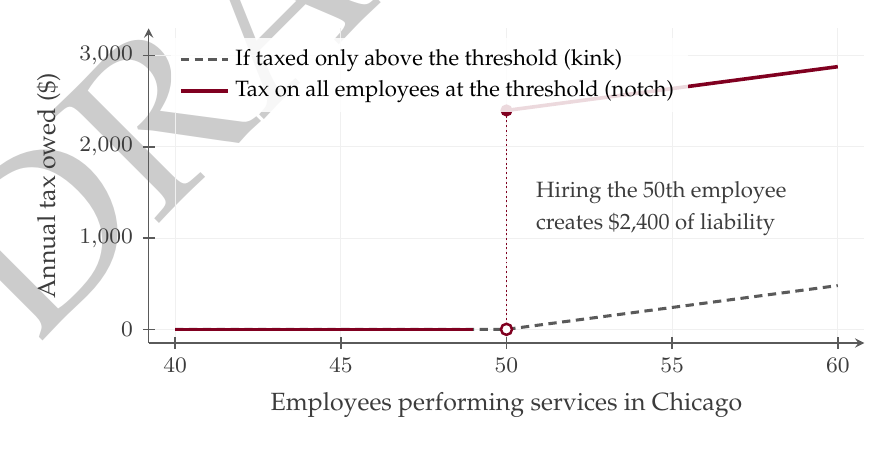
\begin{tikzpicture}
\begin{axis}[
    cmfaxis,
    xlabel={Employees performing services in Chicago},
    ylabel={Annual tax owed (\$)},
    xmin=40, xmax=60, ymin=-150, ymax=3300,
    xtick={40,45,50,55,60},
    legend style={at={(0.03,0.97)}, anchor=north west,
                  font=\footnotesize, draw=none,
                  fill=white, fill opacity=0.85, text opacity=1,
                  cells={anchor=west}},
]
\addplot[cmfgray, line width=1.1pt, densely dashed, mark=none]
    coordinates {(40,0) (50,0) (60,480)};
\addlegendentry{If taxed only above the threshold (kink)}
\addplot[cmfmaroon, line width=1.3pt, mark=none]
    coordinates {(40,0) (49,0)};
\addlegendentry{Tax on all employees at the threshold (notch)}
\addplot[cmfmaroon, line width=1.3pt, mark=none, forget plot]
    coordinates {(50,2400) (60,2880)};
\addplot[cmfmaroon, line width=0.7pt, densely dotted, mark=none, forget plot]
    coordinates {(50,0) (50,2400)};
\addplot[only marks, mark=*, mark size=2pt, forget plot,
         mark options={fill=white, draw=cmfmaroon, line width=0.9pt}]
    coordinates {(50,0)};
\addplot[only marks, mark=*, mark size=2pt, forget plot,
         mark options={fill=cmfmaroon, draw=cmfmaroon}]
    coordinates {(50,2400)};
\node[anchor=west, font=\footnotesize, color=cmfheadergray]
    at (axis cs:50.6,1500) {Hiring the 50th employee};
\node[anchor=west, font=\footnotesize, color=cmfheadergray]
    at (axis cs:50.6,1150) {creates \$2{,}400 of liability};
\end{axis}
\end{tikzpicture}
\caption{A notch, not a kink. Under the Employer's Expense Tax a firm with 49 employees owed nothing, while a firm with 50 owed tax on every employee, producing a discrete jump in liability at the threshold rather than a change in slope. The 50th hire therefore carried the tax cost of the entire workforce, giving firms near the threshold a reason to stay below it. The 500-employee threshold in current proposals has the same structure.}
\label{fig:notch}
\end{figure}

\subsection{Strength and Applicability of the Evidence Base}

The credible quasi-experimental evidence concerns size-contingent labor regulation rather than head taxes as such, and almost none of it is municipal. The results transfer in one respect: notches distort behavior more than their average cost suggests. They transfer poorly in others: the French and Pakistani settings involve national rules, different labor markets and, in the French case, obligations that are not a tax at all. Chicago's tax also applied inside a metropolitan area where a firm can move a worksite across the city line without changing customers or workers, a margin national studies do not have.

\TODO{Document the review method here: what was searched, inclusion criteria, how studies were weighted. State clearly what transfers to Chicago and what does not.}

%% ============================================================
\section{Effects of the 2014 Repeal}
%% ============================================================

\subsection{Empirical Methodology}

\subsubsection{Design}

If employers responded to the 50-employee threshold, the response should be visible in the distribution of employer size. Because the ordinance taxed employers with 50 or more employees, 49 was the last untaxed size, and avoidance predicts excess mass at 49 and a corresponding deficit at and above 50.

Three design choices follow from the institutional setting, and each rules out an alternative that might otherwise seem natural.

\textit{This is a bunching design, not a regression discontinuity.} A regression discontinuity requires that units cannot precisely control which side of the cutoff they fall on. Here they can, and that choice is exactly the object of interest. Describing the design as a regression discontinuity would invite a correct and damaging methodological objection.

\textit{The threshold is a notch, not a kink,} for the reasons set out in Section 3.2. Estimation therefore follows \citet{kleven2013} rather than the kink-based approach of \citet{saez2010}.

\textit{Raw excess mass is not evidence of avoidance.} Business microdata exhibits severe round-number heaping: employers report headcount in round figures, so mass accumulates at 50 and at other round values regardless of whether any threshold is in force. In 2025, when no employment threshold applied anywhere in Illinois, 3,307 Illinois establishments reported exactly 50 employees against 315 at 49 and 344 at 51. Because the heap at 50 leaks into neighboring sizes, a raw spike at 49 cannot be read as avoidance on its own. The design therefore relies on comparison across time, across geographies, and against placebo sizes.

\textit{Statistic and sample.} For a size $k$, we compute
\[
R_k \;=\; \frac{n_k}{\tfrac{1}{6}\left(n_{k-3}+n_{k-2}+n_{k-1}+n_{k+2}+n_{k+3}+n_{k+4}\right)},
\]
the count at $k$ relative to the mean count at nearby sizes, skipping the adjacent size above because the heap at the round number leaks into it. The test size is $k=49$, so the size skipped is 51. Because the count at 51 changes over the panel for reasons we cannot document, we also report the statistic with 51 kept in the baseline, and with each side of 49 used alone (Table~\ref{tab:baselines}). The primary sample consists of single-location establishments with no corporate parent and a verified headcount (data-vendor code ``actual''). This sample is not a deduplication filter, since each establishment appears once per year in every file. It is the sample in which reported headcount can be treated as a firm's headcount, and its limits are discussed below.

\subsubsection{Identification and Statistical Power}

The credibility of a comparative design rests on the comparison areas tracking Chicago in the absence of the policy. We use two comparison areas: suburban Cook County (Cook County outside Chicago) and Illinois outside Cook County. The second is all of Illinois outside Cook, not the collar counties. We report both because they disagree in ways that turn out to be informative.

\textit{Placebo sizes.} The same estimator is run unchanged at twelve other sizes at which no employment threshold applied in Chicago, including 30, 35, 40, 45, 55 and several round numbers from 60 to 90. Their spread is used to calibrate inference, because nominal standard errors from the underlying counts understate the uncertainty. In the placebo exercise, four of twelve placebos were nominally significant at the five percent level on a single-size difference-in-differences test against suburban Cook.

\textit{Detection floor.} The placebo difference-in-differences estimates range from about $-1.2$ to $+1.1$ log points. An effect would need to be roughly as large as tripling the excess at 49 to stand out from that noise. Smaller responses are not ruled out. We have no case in the data in which the estimator is known to detect avoidance where it exists (see the discussion of size 99 below), so this floor is an estimate of noise, not a demonstrated sensitivity.

\subsection{Effects}

\subsubsection{Effects on Employment}

Table~\ref{tab:excess49} reports the excess mass at 49 in Chicago and the two comparison areas by period. Chicago's excess rises from 0.74 in 1998 to 2002 to 4.51 in 2023 to 2025. The clustering at 49 is real. It is not attributable to the tax, for four reasons.

\begin{table}[H]
\centering
\caption{Excess mass at 49 employees ($R_{49}$), single-location observed sample}
\label{tab:excess49}
\small
\begin{tabular}{@{}L{1.05in}L{1.5in}ZZZ@{}}
\toprule
\textbf{Period} & \textbf{Tax regime} & \textbf{Chicago} & \textbf{Suburban Cook} & \textbf{Illinois ex Cook} \\
\midrule
1998--2002 & \$4, threshold 50 & 0.74 & 1.06 & 0.83 \\
2003--2011 & \$4, threshold 50 & 1.74 & \PEND{fill} & \PEND{fill} \\
2012--2013 & Phase-out, \$2 & 2.89 & \PEND{fill} & \PEND{fill} \\
2014--2022 & Repealed & 3.60 & \PEND{fill} & \PEND{fill} \\
2023--2025 & Repealed & 4.51 & 2.27 & 2.14 \\
\bottomrule
\end{tabular}

\vspace{2pt}
{\footnotesize The snapshot month changes from December to July in 2003, so comparisons that cross that date mix policy and data timing. Source: authors' calculations from the Data Axle Historical Business Database. Chicago is city and county both matched to Chicago and Cook.}
\end{table}

\textit{Timing.} On the report's estimator the excess keeps rising through the 2012 rate cut and past the 2014 repeal, and it is highest after the tax is gone. With size 51 kept in the baseline the series peaks in 2011 to 2013, falls in 2014 to 2016 and is back near that level by 2023 to 2025 (Figure~\ref{fig:bunching-lines}). On either baseline the taxed years are no higher than the repealed years when pooled (Table~\ref{tab:baselines}), and avoidance of a tax that no longer exists cannot explain a rise after 2014.

\textit{Untaxed comparison areas.} Suburban Cook and Illinois outside Cook were never subject to the tax, and both show excess mass at 49 that rises over the same years (Table~\ref{tab:excess49}).

\textit{Placebo sizes.} Sizes that carried no threshold are flat across the panel, as Table~\ref{tab:placebo} shows. These placebos have sample sizes comparable to or larger than the sample at 49, so their flatness is not a lack of power.

\begin{table}[H]
\centering
\caption{Excess mass by size, Chicago: first and last period}
\label{tab:placebo}
\small
\begin{tabular}{@{}lZZL{2.6in}@{}}
\toprule
\textbf{Size} & \textbf{1998--2002} & \textbf{2023--2025} & \textbf{Note} \\
\midrule
30 & 0.51 & 0.68 & Placebo \\
35 & 1.13 & 1.08 & Placebo \\
40 & 0.68 & 1.18 & Placebo \\
45 & 0.66 & 0.38 & Placebo \\
\textbf{49} & \textbf{0.74} & \textbf{4.51} & Historical threshold (last untaxed size) \\
55 & 1.24 & 0.55 & Placebo \\
99 & 2.54 & 5.47 & Just below federal WARN Act threshold; see text \\
\bottomrule
\end{tabular}

\vspace{2pt}
{\footnotesize Sizes 60 through 90 are flat or falling and are omitted for space. Source: authors' calculations.}
\end{table}

\textit{Magnitude.} The excess at 49 in Chicago amounts to about 89 businesses across the nine taxed years from 2003 to 2011, or about 10 a year citywide, against roughly 2,200 firms paying the tax annually. After repeal it is about 210 businesses over nine years, or about 23 a year. With size 51 kept in the baseline the figures are about 90 businesses (10 a year) in the taxed years and about 151 (17 a year) after repeal. On either baseline the excess is larger once the tax is gone (Figure~\ref{fig:bunching-bars}).

\paragraph{Formal inference.} Because nominal standard errors over-reject, we base inference on the placebo distribution. Table~\ref{tab:inference} shows that no specification is significant on that basis. The nominal difference-in-differences estimates of $-0.328$ against suburban Cook and $-0.286$ against Illinois outside Cook are negative, meaning the gap between Chicago and its controls widened after repeal, which is the opposite of what avoidance predicts. The sign also depends on the choice of pre and post windows, which is a further reason not to rely on the difference-in-differences.

\begin{table}[H]
\centering
\caption{Placebo-based inference on the difference-in-differences at 49}
\label{tab:inference}
\small
\begin{tabular}{@{}L{2.0in}ZZZ@{}}
\toprule
\textbf{Specification} & \textbf{Estimate} & \textbf{Placebos at least as large} & \textbf{Placebo $p$} \\
\midrule
Size 49 vs suburban Cook & $-0.328$ & 7 of 12 & 0.58 \\
Size 49 vs Illinois ex Cook & $-0.286$ & 2 of 12 & 0.17 \\
Sizes 46--49 pooled vs suburban Cook & $+0.004$ & \PEND{count} & 1.00 \\
Sizes 46--49 pooled vs Illinois ex Cook & $-0.179$ & \PEND{count} & 0.67 \\
\bottomrule
\end{tabular}

\vspace{2pt}
{\footnotesize Estimates are in log points, 2003--2011 versus 2014--2022. Source: authors' calculations.}
\end{table}

\paragraph{Trends.} Firms may adjust slowly to a standing threshold, which would show up as growth in excess mass while taxed and a plateau after repeal. Table~\ref{tab:trends} tests trends directly. Chicago's excess grows at 0.123 a year during 2003 to 2011 and only 0.015 a year after 2014. Suburban Cook shows the same deceleration, while Illinois outside Cook accelerates. The two comparison areas therefore disagree with each other, and the divergence is between Cook County and downstate, not between Chicago and everywhere else. A tax levied only inside the city cannot produce a pattern that suburban Cook shares. The difference in trends against suburban Cook is small and insignificant on the placebo distribution ($p=0.67$). We therefore treat suburban Cook as the more relevant comparison.

\begin{table}[H]
\centering
\caption{Trend in excess mass at 49, taxed versus repealed years}
\label{tab:trends}
\small
\begin{tabular}{@{}L{1.9in}ZZZ@{}}
\toprule
\textbf{Area} & \textbf{Trend, 2003--2011} & \textbf{Trend, 2014--2022} & \textbf{Change} \\
\midrule
Chicago & $+0.1226$ & $+0.0153$ & $-0.107$ \\
Suburban Cook & $+0.0557$ & $-0.0029$ & $-0.059$ \\
Illinois ex Cook & $+0.0098$ & $+0.0558$ & $+0.046$ \\
\midrule
\multicolumn{4}{@{}l}{\textbf{Difference in trends (Chicago minus control)}} \\
\quad vs suburban Cook & \multicolumn{3}{l}{$+0.0488$, placebo $p=0.67$} \\
\quad vs Illinois ex Cook & \multicolumn{3}{l}{$+0.1534$ [$+0.0569$, $+0.2499$], placebo $p=0.17$} \\
\bottomrule
\end{tabular}

\vspace{2pt}
{\footnotesize Trend is the annual change in $R_{49}$. Brackets give the nominal 95 percent interval, which over-rejects. Source: authors' calculations.}
\end{table}

\figslot{fig7_bunching_lines}{Clustering at 49 employees in Chicago, Cook County outside Chicago and Illinois outside Cook County, 1998 to 2025. The left panel leaves size 51 out of the baseline, as the report's estimator does; the right panel keeps it in.}{fig:bunching-lines}{Two-panel line graph. R at 49 by year for three areas, tax years shaded. Left panel skips size 51 in the baseline, right panel keeps it. File: fig7\_bunching\_lines.pdf.}

\begin{table}[H]
\centering
\caption{Sensitivity of the excess at 49 to the baseline, Chicago}
\label{tab:baselines}
\small
\begin{tabular}{@{}L{3.0in}ZZ@{}}
\toprule
\textbf{Baseline sizes} & \textbf{Taxed, 2003--2011} & \textbf{Repealed, 2014--2022} \\
\midrule
46--48 and 52--54 (report estimator, 51 left out) & 1.74 & 3.60 \\
46--48 and 51--54 (51 kept in) & 1.77 & 2.08 \\
46--48 only & 1.52 & 3.72 \\
52--54 only & 2.04 & 3.49 \\
\bottomrule
\end{tabular}

\vspace{2pt}
{\footnotesize Ratio of the count at 49 to the average count at the baseline sizes, single-location observed sample. Size 50 is excluded from every baseline. Source: authors' calculations.}
\end{table}

\figslot{fig1_bunching}{Chicago businesses at each reported size from 46 to 54, pooled over the taxed years (2003 to 2011) and the repealed years (2014 to 2022). The dashed line is the average of the neighbouring sizes, with 51 included.}{fig:bunching-bars}{Two-panel bar chart of counts at sizes 46 to 54, with 50 truncated and the baseline line. File: fig1\_bunching.pdf.}

\paragraph{What we cannot claim.} Four concessions bear on how the null should be read.

First, there is no positive control. Size 99, just below the federal WARN Act threshold of 100, shows a high excess in all three areas, but more businesses sit just above 100 than just below it, so the high value reflects spillover from the heap at 100 and not avoidance. The method has therefore not been shown to detect avoidance where it exists.

Second, reported headcounts cannot distinguish a firm that stays at 49 employees from a firm that reports 49. Both responses are threshold-driven and neither is specific to Chicago, so the conclusion stands, but we have not measured employment decisions.

Third, Chicago's excess rose 2.4-fold from 2003 to 2011 while the rate and threshold were fixed, and that rise is unexplained, although suburban Cook shows a smaller one. Both the series at 49 and at 99 begin rising around 2002 to 2003, which is also when the snapshot month moves from December to July and the modeled-employment codes change (Appendix A). We state the level as real and the timing of its increase as unaccounted for.

Fourth, one pattern looks like avoidance and is not. The asymmetry between counts at 49 and 51 in Chicago peaks at the 2012 to 2013 phase-out and turns negative after repeal, which reads like avoidance ending when the tax ends. The count at 51 rises from 107 in 2003 to 2011 to 491 in 2014 to 2022, and we cannot document why. The rise comes from records first added to the file in 2013 and visible from the 2014 files: among records still in the 2025 file that first appeared in 2013 and sit in the 50 to 99 band, 22 of 58 (38 percent) report exactly 51, against 23 of 1,155 (2 percent) for all other entry years. Six of the 2013 records at 51 carry no phone-verification date. A default headcount on newly added records would produce this pattern, but the vendor documentation available to us does not say so, and we treat that as a hypothesis, not a finding. We neither adjust the count at 51 nor use the pattern as evidence. Instead we report the excess at 49 with 51 left out of the baseline and kept in it (Table~\ref{tab:baselines}), and the conclusion does not depend on the choice.

\figslot{bunching_asymmetry}{Asymmetry between counts at sizes just below and just above each threshold, by period.}{fig:asymmetry}{Optional diagnostic. Log ratio of counts at R-1 and R+1 for sizes 49 and 99 in Chicago, showing the jump in the count at 51. Generated by 29\_bunching\_diagnostics.py.}

\subsubsection{Effects on Wages}

The business microdata underlying this report records establishment employment and sales volume but not payroll, so we do not estimate wage effects directly. Two forms of evidence bear on the question.

Descriptively, Bureau of Labor Statistics data indicate that Illinois workers at businesses with 500 or more employees are paid more on average than counterparts at smaller establishments, though the Bureau does not publish size-class breakdowns at the city or county level \citep{woelfel2025}. Any head tax with a large-employer threshold therefore falls disproportionately on comparatively well-paid jobs.

Theoretically, the incidence literature summarized in Section 3 holds that a per-employee levy is likely absorbed by employers in the short run and shifted toward labor over longer horizons through slower wage growth. Chicago's tax was small enough relative to compensation that any such shift would be difficult to detect against normal wage variation.

\TODO{Confirm with Marlowe whether this subsection stays at this scope or folds into Implications.}

\subsubsection{Effects on Business Location/Relocation}

\TODO{Scope decision needed. A credible estimate requires a border-discontinuity design comparing establishments immediately inside and outside the city line. The geocoding supports it: match codes are parcel or site level on 91.3 percent of Illinois records, and excluding ZIP-centroid matches costs about 6.5 percent of Chicago rows. It is a separate build and unlikely to fit this cycle. Fallback is descriptive relocation evidence plus the literature. Note that the comparison with suburban Cook in the bunching results is informative about relocation only indirectly.}

\subsection{Implications}

Three points follow from the historical evidence.

First, the tax Chicago had was too small to produce a detectable behavioral response, and a null is the economically expected result. Crossing the 50-employee threshold cost about \$2,400 a year, roughly 0.1 percent of the payroll of a fifty-person firm. A null is also consistent with the WBEZ finding of no causal link between the tax and job loss \citep{woelfel2025}.

Second, the null does not transfer. The proposed tax has a notch of about \$198,000, two orders of magnitude larger. Nothing in the historical record lets us infer how employers would respond at that scale.

Third, the historical test observes only single-location businesses, because multi-site firms cannot be treated as having a single reported headcount. A 500-employee threshold reaches a population that is mostly multi-site: 185 of the 243 firms in our central base, holding 83 percent of its employment. This is a structural reason the historical test does not speak to the current proposal, and it is why the base erosion question in Section 5.3 remains open. Figure~\ref{fig:thresholds} sets the two populations side by side.

\figslot{fig5_threshold_comparison_50_vs_500}{Chicago employers reached by the old 50-employee threshold and by a 500-employee threshold, 2025, by corporate parent.}{fig:thresholds}{Table-style exhibit comparing 50+ and 500+ on firms, employment, median size, locations, sales, portable-sector share and verification. File: fig5\_threshold\_comparison\_50\_vs\_500.pdf.}

What a null does not establish is that the tax is costless. Base erosion can occur without employment loss, which is the subject of Section 5.3.

%% ============================================================
\section{Likely Effects of a Head Tax Today}
%% ============================================================

\subsection{Head Tax Base}

\subsubsection{Data and Measurement}

The analysis uses the Data Axle Historical Business Database, formerly InfoGroup, licensed through the University of Chicago Library for non-commercial academic use. The panel covers 1997 to 2025, and every year used is from the same full-file product tier, so there is no mid-panel product switch. The file records individual establishments with location, employment, industry, and, critically for this report, an identifier linking each establishment to its corporate parent. Aggregate results only are reported.

Four properties of the data constrain what can be claimed, and all are documented in Appendix A.

\textit{Composition changes over time.} Between 2011 and 2025 the count of Chicago establishments in the file rose by 22 percent, from 113,532 to 139,025, while total Chicago employment in the file fell by 3.2 percent and the number of records carrying verified employment fell by 27 percent (Table~\ref{tab:composition}). The growth in record counts reflects the vendor adding small, low-employment modeled records, not growth in Chicago business activity. One example illustrates the scale: the single largest Chicago parent in the 2025 file is the U.S.\ Postal Service, with 2,187 establishments, of which 2,121 are collection boxes with no employment. Any descriptive claim about business formation drawn from the full sample would be mistaken. Results are therefore reported on the sample with observed employment wherever the distinction matters.

\begin{table}[H]
\centering
\caption{Chicago in the Data Axle file, 2011 and 2025}
\label{tab:composition}
\small
\begin{tabular}{@{}L{2.6in}QQ@{}}
\toprule
 & \textbf{2011} & \textbf{2025} \\
\midrule
Establishments & 113,532 & 139,025 \\
Total employment & 1,417,304 & 1,371,766 \\
Records with verified (observed) employment & 54,128 & 39,727 \\
\quad Share of establishments & 47.7\% & 28.6\% \\
Employment missing & 1.67\% & 7.01\% \\
Firms with more than one Chicago establishment & 1.0\% & 1.2\% \\
\bottomrule
\end{tabular}

\vspace{2pt}
{\footnotesize Source: authors' calculations. Employment missing is the share of records with the vendor's zero code recoded to missing.}
\end{table}

\textit{Verification rises with size.} The share of records with verified employment increases steeply with establishment size, and reaches 100 percent above 500 employees (Table~\ref{tab:verified-share}). Restricting to verified records therefore costs little in the size range where the tax binds. Across the central base of firms at 500 or more employees, 90.1 percent of employment comes from verified records (Section 5.1.3).

\begin{table}[H]
\centering
\caption{Share of Chicago establishment records with verified employment, by size, 2025}
\label{tab:verified-share}
\small
\begin{tabular}{@{}lC{1.2in}@{}}
\toprule
\textbf{Size band} & \textbf{Verified share} \\
\midrule
1 to 4 & 16.4\% \\
5 to 9 & 45.3\% \\
10 to 19 & 59.1\% \\
20 to 49 & 64.1\% \\
Exactly 50 & 93.2\% \\
51 to 99 & 59.8\% \\
100 to 249 & 79.4\% \\
250 to 499 & 98.3\% \\
500 and over & 100.0\% \\
\midrule
All Chicago records & 28.6\% \\
\bottomrule
\end{tabular}

\vspace{2pt}
{\footnotesize Source: authors' calculations.}
\end{table}

\textit{A floor at one employee.} In 2025, 47,107 Chicago records (34 percent) report exactly one employee, and 92 percent of them are modeled. This looks like a default and not an estimate. It has little effect on the bunching analysis, since modeled records sit far from 50, but genuinely larger unverified firms could sit at one employee and be missed. The verified share above shows the tax base itself is largely unaffected. \PEND{Benchmark total and size-class employment against QCEW and SUSB before any figure goes to the client. The 2025 Cook County employment figure of 2,639,708 runs above IDES QCEW private employment for Cook and requires reconciliation.}

\textit{Geography and heaping.} The file's city field drifted between years: in 2011 no record carried a Chicago city name with a county outside Cook, while 2025 has 1,367. The Chicago filter therefore requires both city and county. Employers also report headcount in round numbers, so the excess at 50 seen in any single year is not by itself informative, as set out in Section 4.

All figures are to be benchmarked against the Quarterly Census of Employment and Wages, the Census Bureau's Statistics of U.S.\ Businesses and LEHD Origin-Destination data, and the Illinois Department of Employment Security's \textit{Where Workers Work} series. \PEND{report the benchmark comparison}

\subsubsection{From Establishments to Firms}

Section 2.1 established that Chicago's ordinance taxed employers according to their Chicago employment. Published statistics do not report that quantity. The Bureau of Labor Statistics defines an establishment as a single economic unit at one physical location, in contrast to a firm, which may comprise many establishments \citep{bls2025}. A count of establishments with 500 or more employees therefore counts large worksites, not large employers. The Census Bureau's firm-size measure has the opposite problem, reporting national firm size rather than Chicago employment, and so overstates the base.

The parent identifier in the business microdata permits a measure that matches the ordinance. Establishments are first restricted to Chicago, and then aggregated to their corporate parent, so that each firm carries only the employment located within the city. Single-location establishments with no parent are treated as firms in their own right. The result is a distribution of employer size measured as the Department of Revenue would have measured it (Appendix B).

For small employers the distinction turns out not to matter much: only 1.0 percent of Chicago firms in 2011 and 1.2 percent in 2025 have more than one Chicago establishment. For large employers it matters a great deal, which is why the rollup is essential for the 500-employee threshold.

The measure has known limitations, and they mostly run in one direction. The parent identifier captures corporate parent and subsidiary structure. It does not link several separately incorporated entities held by the same individuals, which is precisely the arrangement that Employer's Expense Tax Ruling No.~2 combined and that the court upheld in \textit{DTCT} \citep{dtct2011}. Those structures appear in the data as unrelated single-location businesses. The parent identifier is also fragmented in some sectors. Northwestern Medicine appears as 218 establishments spread across 193 parent identifiers, and other hospital systems show the same pattern, so health care is understated in the base. We do not merge these systems, and we state the understatement as a limitation of the base and not as a correction applied to it. The firm-level base reported here is therefore, on balance, a \textbf{lower bound} on the population that would be liable, with the shortfall concentrated in hospital systems, franchised retail, food service, staffing and home health care.

Two further data problems at the top of the distribution matter because they feed revenue directly. Some large employers report round figures (8,000, 7,000, 5,000) that drive revenue: a firm reporting 5,000 employees instead of 3,200 adds about \$712,000. And some records carry a company-wide headcount on a single Chicago establishment. Section 5.1.3 describes the rules we use to screen for both and reports the base with and without the weaker of them.

\subsubsection{Estimates of the Liable Base}

We build the base in stated steps, each of which can be checked in the data. Table~\ref{tab:base-build} reports what each step removes.

\begin{table}[H]
\centering
\caption{Construction of the 2025 taxable base at a threshold of 500 Chicago employees}
\label{tab:base-build}
\small
\begin{tabular}{@{}L{3.6in}C{0.8in}C{0.9in}@{}}
\toprule
\textbf{Step} & \textbf{Firms} & \textbf{Employees} \\
\midrule
All firms at 500 or more Chicago employees & 284 & 461,281 \\
\quad Less government: NAICS 92 & $-14$ & $-19,196$ \\
\quad Less government: named public bodies not caught by NAICS & $-19$ & $-34,959$ \\
\textbf{Upper base} & \textbf{251} & \textbf{407,126} \\
\quad Less Rule A: company-wide headcount on a single site & $-8$ & $-18,790$ \\
\textbf{Central base} & \textbf{243} & \textbf{388,336} \\
\quad Less Rule B: rollup above vendor corporate total & $-11$ & $-53,516$ \\
\quad Less Rule C: franchise pattern & $-1$ & $-5,918$ \\
\quad Less review: large single-site firms with no parent record & $-17$ & $-35,505$ \\
\textbf{Conservative base} & \textbf{214} & \textbf{293,397} \\
\bottomrule
\end{tabular}

\vspace{2pt}
{\footnotesize Source: authors' calculations from the Data Axle Historical Business Database. Firms are corporate parents measured by Chicago employment; establishments with no parent are their own firm.}
\end{table}

\textit{Government.} Government employers are removed first because this is a legal constraint and not a policy choice: a city cannot tax its own departments, and federal and state bodies are beyond municipal reach. The vendor codes many public bodies to their operating industry, so the Transit Authority appears as transportation and the Streets Department as construction. We therefore identify government by industry code (NAICS 92) and by a named list of public bodies. The name list is the one judgment-based part of the screen and is reproduced in the methods appendix.

\textit{Screens on doubtful headcounts.} Rule A removes a single-location firm that reports more employees than its own parent record. With one Chicago site, the site and the parent record should carry the same headcount, so a gap means a company-wide figure was written onto a local record. Examples are one professional services firm at 4,036 against 500 on its parent record, and one asset manager at 7,000 against 3,500. Rule A is arithmetic and involves no judgment about names, so it defines the central base. Three weaker screens define the conservative base. Rule B removes firms whose Chicago rollup exceeds the vendor's corporate total, where one exists. That field is populated for only about a quarter of large firms and is sometimes stale. Rule C removes a franchise pattern, meaning 100 or more locations, an average under 15 employees per location, and a rollup more than ten times the parent record. Franchisees are separately owned, so they are not one employer under the common-ownership test. The last screen flags large single-site firms with no parent record, where no test can be run. They are flagged and removed only from the conservative base, not judged.

\textit{Composition.} On the central base, health care accounts for 16.8 percent of employment, professional and technical services for 14.4 percent, accommodation and food for 10.3 percent, finance and insurance for 9.8 percent, retail for 9.7 percent and education for 7.5 percent. Figure~\ref{fig:industry} shows the base by sector, with the share of each sector's workforce that usually works from home.

\figslot{fig2_industry_remote}{Central base by sector: Chicago employees at firms with 500 or more employees, the share removed by the remote-work adjustment, and the metropolitan work-from-home rate with the portability tiers.}{fig:industry}{Two-panel figure: bars of employees by sector with the remote-adjusted share in orange, and work-from-home rate by sector colored by portability tier. File: fig2\_industry\_remote.pdf.}

\textit{Verified employment.} Across the central base, 90.1 percent of employment comes from records with verified headcounts, against 28.6 percent of all Chicago establishment records (Table~\ref{tab:observed-base}). The one-employee floor described above therefore has little effect on the tax base.

\begin{table}[H]
\centering
\caption{Share of central-base employment from verified records, by firm type}
\label{tab:observed-base}
\small
\begin{tabular}{@{}lC{0.9in}C{0.9in}@{}}
\toprule
\textbf{Chicago establishments per firm} & \textbf{Firms} & \textbf{Verified share} \\
\midrule
1 & 58 & 100.0\% \\
2 to 10 & 113 & 96.2\% \\
11 to 50 & 46 & 82.4\% \\
More than 50 & 26 & 78.2\% \\
\midrule
All central-base firms & 243 & 90.1\% \\
\bottomrule
\end{tabular}

\vspace{2pt}
{\footnotesize Source: authors' calculations.}
\end{table}

Moving from the liable population to the taxable base requires several further restrictions, which we report separately so that the effect of each is visible: the treatment of nonprofit and other employers under an exemption schedule, full-time status, and the requirement that an employee perform at least half of their services within the city. Section 5.2 takes them in turn.

\TODO{The nonprofit question is a live scoping decision, not an analytical one. The Civic Committee has an interest in whether large hospitals and cultural institutions are included, and the answer materially changes the base. Confirm with Mary Wagoner and report the base with and without.}

\subsection{Estimates of Potential Revenue}

\subsubsection{Our Estimate}

No exemption schedule was ever published for the proposal, so every exemption tier below is an assumption of ours and is labelled as such. Turning the liable base into revenue takes three steps, and every parameter in them comes from our firm-level base or from a public Census table.

\textit{Exemption tiers.} Government is already removed. The tiers then exempt, cumulatively, education; education and hospitals; education and all health care; and education, all health care, and civic and religious employers. The last is the narrowest base.

\textit{Two readings of the tax.} Reading A applies the tax to every employee, which is how coverage of the Mayor's proposal describes it. Reading B applies it only to full-time employees, as the historical ordinance did, and multiplies covered employees by a full-time share of 0.7839. That share is the fraction of workers in the Chicago metropolitan area who usually work 35 or more hours a week, from American Community Survey table B23022 (2024, one-year).

\textit{Remote-work adjustment.} A remote worker who lives in Chicago still works in Chicago, so only remote workers who live outside the city can fall outside the tax. For each firm we compute
\[
\text{escaping employees} \;=\; \text{employees} \times w_s \times (1-\rho),
\]
where $w_s$ is the metropolitan work-from-home rate for the firm's industry group (table B08126) and $\rho=0.6926$ is the share of jobs in Chicago held by Chicago residents (1,085,613 of 1,567,413, tables B08008 and B08604). The industry rates range from 6.9 percent in arts, accommodation and food to 31.0 percent in professional, scientific and management services, and are 14.9 percent across all industries (Appendix C). Each firm is then re-tested against the 500-employee threshold on its adjusted headcount, and a firm that drops below 500 leaves the base. We report three cases: unadjusted, the Census adjustment above, and a lower bound in which every remote worker lives outside the city ($\rho=0$).

Table~\ref{tab:revenue} reports the central case: the central base with the Census adjustment, at \$396 per employee per year.

\begin{table}[H]
\centering
\caption{Estimated annual revenue at \$396 per employee, central base with Census remote-work adjustment}
\label{tab:revenue}
\small
\begin{tabular}{@{}L{2.5in}ZZZ@{}}
\toprule
\textbf{Exemption scenario} & \textbf{Firms} & \textbf{Reading A: all employees (\$M)} & \textbf{Reading B: full-time only (\$M)} \\
\midrule
Government removed only & 218 & 141.2 & 110.7 \\
Less education & 208 & 130.3 & 102.2 \\
Less education and hospitals & 193 & 114.2 & 89.5 \\
Less education and all health care & 183 & 105.6 & 82.8 \\
Less education, all health care, civic and religious (narrowest) & 176 & 103.2 & 80.9 \\
\bottomrule
\end{tabular}

\vspace{2pt}
{\footnotesize Source: authors' calculations from the Data Axle Historical Business Database and American Community Survey 2024 one-year tables. Covered employees under Reading A range from 356,587 (government removed only) to 260,612 (narrowest); under Reading B from 279,523 to 204,290.}
\end{table}

Table~\ref{tab:sensitivity} shows how much the answer depends on the base and on the adjustment, for the widest and narrowest exemption tiers.

\begin{table}[H]
\centering
\caption{Sensitivity of annual revenue to the base and the remote-work adjustment (\$ millions)}
\label{tab:sensitivity}
\footnotesize
\begin{tabular}{@{}L{0.95in}L{0.8in}*{6}{>{\Centering\arraybackslash}p{0.52in}}@{}}
\toprule
 & & \multicolumn{3}{c}{\textbf{Reading A}} & \multicolumn{3}{c}{\textbf{Reading B}} \\
\cmidrule(lr){3-5}\cmidrule(lr){6-8}
\textbf{Base} & \textbf{Tier} & \textbf{None} & \textbf{Census} & \textbf{All out} & \textbf{None} & \textbf{Census} & \textbf{All out} \\
\midrule
Upper & Widest & 161.2 & 147.9 & 123.8 & 126.4 & 116.0 & 97.1 \\
Upper & Narrowest & 121.2 & 109.9 & 88.8 & 95.0 & 86.2 & 69.6 \\
Central & Widest & 153.8 & 141.2 & 118.3 & 120.5 & 110.7 & 92.7 \\
Central & Narrowest & 113.7 & 103.2 & 83.3 & 89.2 & 80.9 & 65.3 \\
Conservative & Widest & 116.2 & 105.3 & 86.4 & 91.1 & 82.6 & 67.7 \\
Conservative & Narrowest & 97.5 & 88.0 & 70.6 & 76.4 & 69.0 & 55.3 \\
\bottomrule
\end{tabular}

\vspace{2pt}
{\footnotesize Source: authors' calculations. None: no remote-work adjustment. Census: adjustment with the Census resident share. All out: every remote worker lives outside Chicago. Widest tier removes government only; narrowest also removes education, all health care, and civic and religious employers.}
\end{table}

On the central base with the Census adjustment, revenue runs from \$80.9 million to \$141.2 million. Across all three bases and both adjusted cases it runs from \$55.3 million to \$147.9 million. Two features of the estimate matter for how it should be read. First, the adjustment moves 25 firms in the central base out of the 500-employee base, and nearly all of them, 96 percent, have 550 employees or fewer. If every remote worker lived outside the city, 58 firms would drop out. The estimate is therefore sensitive to how many employers sit close to the threshold (Figure~\ref{fig:near500}). Second, the adjusted figures are not conservative in one direction only. The Census category counts workers who worked from home most days of the survey week. Under wording like that of the historical ordinance, which reached work performed ``in whole or in part'' within the city, some of those workers come in occasionally and would still be taxable, so the adjustment understates revenue. Against that, the point-in-time snapshot and perfect compliance overstate it.

\figslot{fig6_firms_near_500}{Chicago firms with 400 to 700 employees, 2025, in 10-employee bins. Ten firms report exactly 500.}{fig:near500}{Histogram of firms near the 500 threshold with the threshold marked. File: fig6\_firms\_near\_500.pdf.}

Two limitations follow from using public data. The work-from-home rates are metropolitan averages for each industry, applied to individual firms, and the resident share is a citywide average. Neither is measured firm by firm.

Table~\ref{tab:assumptions} lists the assumptions that could move these figures and the direction each pushes.

\begin{table}[H]
\centering
\caption{Assumptions in the revenue estimate and the direction of their effect}
\label{tab:assumptions}
\small
\begin{tabular}{@{}L{3.3in}L{1.5in}@{}}
\toprule
\textbf{Assumption} & \textbf{Direction} \\
\midrule
Point-in-time snapshot stands in for a tax assessed monthly & Overstates \\
Perfect compliance, no behavioral response & Overstates \\
A qualifying firm pays on all employees, not only those above the threshold & Overstates if only those above \\
Threshold counts Chicago employees, not company-wide employees & Understates if company-wide \\
Parent identifiers fragment some firms, mostly hospital systems & Understates \\
Remote workers counted as escaping only if they live outside Chicago & Understates if some come in occasionally \\
Industry work-from-home rates and resident share are averages, not firm-specific & Uncertain \\
Vendor-modeled employment inside firm totals (about 10 percent of the base) & Uncertain \\
Full-time share is a metropolitan average and not the wage-based ordinance definition & Uncertain \\
\bottomrule
\end{tabular}
\end{table}

\figslot{fig3_revenue_range}{Estimated annual revenue by exemption scenario and reading of the tax, central base, with no remote adjustment, the Census central case and the bounding case, compared with the Administration's projection of \$82 million.}{fig:revenue}{Two-panel bar chart. Every employee and full-time only, five exemption tiers, three remote-work cases, vertical reference line at \$82 million. File: fig3\_revenue\_range.pdf.}

Figure~\ref{fig:rates} shows how the central case scales with the rate, since revenue is proportional to it.

\figslot{fig4_revenue_by_rate}{Annual revenue by exemption tier and tax rate, central base with the Census remote-work adjustment.}{fig:rates}{Two grids of revenue by exemption and rate (\$33, \$40, \$50, \$60, \$75 per month), Reading A and Reading B. File: fig4\_revenue\_by\_rate.pdf.}

\subsubsection{Comparison with the City's Estimates}

Table~\ref{tab:compare} sets our base beside the Administration's public projection and the historical record.

\begin{table}[H]
\centering
\caption{Comparison of firm counts, covered employees and revenue}
\label{tab:compare}
\small
\begin{tabular}{@{}L{2.5in}ZZZ@{}}
\toprule
\textbf{Source} & \textbf{Firms} & \textbf{Covered employees} & \textbf{Revenue (\$M)} \\
\midrule
Administration's projection & about 175 & about 207,070 & 82.0 \\
WBEZ, average 2000--2013 (paid the tax, 500 or more) & about 188 & about 225,000 & -- \\
This report, government removed only, Reading A & 218 & 356,587 & 141.2 \\
This report, narrowest exemptions, Reading A & 176 & 260,612 & 103.2 \\
This report, narrowest exemptions, Reading B & 176 & 204,290 & 80.9 \\
\bottomrule
\end{tabular}

\vspace{2pt}
{\footnotesize Sources: WBEZ \citep{woelfel2025}; the Administration's figures as reported publicly; authors' calculations. The Administration's covered-employee figure is implied by \$82 million at \$396 per employee. Our figures use the central base with the Census adjustment.}
\end{table}

The Administration's figures sit at the bottom of our range. Only in our narrowest scenario under Reading B, with 176 firms, 204,290 covered employees and \$80.9 million, do our figures match theirs of about 175 firms, 207,070 employees and \$82.0 million. We do not read that match as evidence about how the Administration built its number. No exemption schedule was published, and several combinations of exemptions and readings can land on the same total. What the comparison does show is that under Reading A our covered-employee counts exceed the Administration's by 26 percent (narrowest exemptions) to 72 percent (government removed only). The WBEZ historical figure, about 225,000 jobs at 188 firms, is closer to the Administration's number than to our broader scenarios.

Three explanations for the gap are worth distinguishing. The projection may embed an exemption schedule at least as narrow as our narrowest. It may apply the tax only to full-time employees, as the historical ordinance did. Or it may reflect data that are a decade old, as a senior policy official has acknowledged.

\subsection{Behavioral Effects}

This section sets out the report's principal conclusion about the current proposal.

The proposed structure retains the notch design of the historical tax and enlarges it considerably. At \$396 per employee per year with a threshold of 500, an employer at 499 Chicago employees owes nothing and an employer at 500 owes \$198,000. A single hire carries that entire liability. Expressed against total compensation for 500 employees the amount is small, but the incentive created by a notch does not scale with the tax's share of costs. It scales with the discontinuity itself, which is what firms observe when deciding whether to stay below it.

The literature reviewed in Section 3.2 is direct on this point: notches induce large behavioral responses even where the underlying structural elasticity is modest \citep{kleven2013}. The relevant margins for a Chicago employer are not primarily hiring decisions. They include assigning employees to suburban locations, reclassifying workers as contractors or part-time, expanding remote arrangements so that fewer employees perform half or more of their services within the city, and reorganizing corporate structure. The last of these is what the Department of Revenue was contending with in 2005, and the \textit{DTCT} litigation demonstrates both that firms pursue it and that the city can contest it only through enforcement action.

The implication for the revenue estimate is that a static base is the wrong assumption. Any estimate for the current proposal, including ours, applies a tax rate to a base measured before the tax exists. The literature gives no basis for expecting that base to be stable. It also suggests that the firms best positioned to restructure are the largest and most sophisticated, which means the burden that remains falls on employers with the least capacity to reorganize.

We cannot estimate the erosion rate from history. The historical test found no detectable response, but it could only have detected a large one, it observes only single-site firms, and it covers a notch two orders of magnitude smaller than the one proposed. We can, however, show how little erosion it would take to change the fiscal picture. Table~\ref{tab:erosion} applies illustrative erosion rates to four of our central estimates and reports the rate at which revenue falls to the Administration's \$82 million. Under Reading A, erosion of 21 to 42 percent of the base is enough. Under Reading B on the narrowest exemptions, our estimate is already below \$82 million before any erosion. Revenue is treated as proportional to the base, which is an approximation: a firm that restructures below the threshold removes all of its employment at once. These are illustrations of the sensitivity, not forecasts.

\begin{table}[H]
\centering
\caption{Illustrative effect of base erosion on annual revenue (\$ millions)}
\label{tab:erosion}
\footnotesize
\begin{tabular}{@{}L{1.9in}*{5}{>{\Centering\arraybackslash}p{0.62in}}@{}}
\toprule
\textbf{Central estimate} & \textbf{No erosion} & \textbf{10\%} & \textbf{20\%} & \textbf{30\%} & \textbf{Erosion to reach \$82M} \\
\midrule
Reading A, government removed only & 141.2 & 127.1 & 113.0 & 98.8 & 42\% \\
Reading A, narrowest exemptions & 103.2 & 92.9 & 82.6 & 72.2 & 21\% \\
Reading B, government removed only & 110.7 & 99.6 & 88.6 & 77.5 & 26\% \\
Reading B, narrowest exemptions & 80.9 & 72.8 & 64.7 & 56.6 & already below \\
\bottomrule
\end{tabular}

\vspace{2pt}
{\footnotesize Erosion is the share of the taxable base lost to restructuring, relocation of employees, or reclassification. Illustrative arithmetic only.}
\end{table}

%% ============================================================
\section{Conclusion}
%% ============================================================

\TODO{Write last. Do not introduce new evidence. Restate the finding, name the decision it bears on, and be clear about what the analysis cannot settle. Points to carry: historical null and why it does not transfer; our estimates bracket the Administration's \$82 million, near the bottom of the range; static base is the wrong assumption; no peer-reviewed causal evidence on U.S. municipal head taxes; the caveats on the remote-work adjustment (averages, not firm-specific).}

%% ============================================================
\appendix
%% ============================================================

\section{Data Provenance and Quality}

\TODO{Licensing and terms.} The panel is licensed through the University of Chicago Library for non-commercial academic use, and the project's principal investigator has confirmed use and sharing for this project. Vendor documentation is available from public library sources.

\subsection*{File layout and delivery seams}

Each year is delivered as two members, A and B, with 89 fields. Illinois records for 2025 are all in member A. The panel spans 29 years (1997 to 2025), and several seams matter for any analysis of change over time.

\begin{itemize}[leftmargin=*,itemsep=2pt]
\item The 1997 to 2000 files have no header line and pad every line with trailing spaces; 2002 member A is headerless while B has a header. The standard column names were applied and alignment verified on every row.
\item Several years contain malformed quoting, which was repaired and logged, not dropped: 85 lines in 2023, 3 in 2024, and 1 each in 1997 and 1998.
\item The 1997 file has no usable observed flag and is excluded from anything that uses the verified sample.
\item From 1998 to 2002 single-location businesses carry a parent number of zero and blank status, recoded to no parent. In those years, records modeled by industry code carry only a size band, so employment is missing on 18 to 24 percent of records.
\item The snapshot month is December for 1997 to 2002 and July from 2003.
\item Modeled-employment codes change over time: one code is large from 1998 to 2002, another appears in 2003, the industry-modeled code is absent from 2007 to 2015 and returns from 2016 to 2022, the professional-modeled code surges in 2013, and from 2023 only actual and professional-modeled records exist.
\item The share of Chicago records with verified employment falls from about 66 percent in 1998 to 48 percent in 2011, 32 percent in 2022 and 29 percent in 2025.
\end{itemize}

\subsection*{The zero sentinel}

Missing employment appears in the raw file as the code 00000, not as a blank. Casting it directly to a number produces zero, not missing, so it was recoded explicitly, and the recode was verified against a second independent field (the vendor's employment size band, which is blank on exactly the same rows). In 2025, 7.34 percent of Illinois records carry the sentinel.

\subsection*{Composition finding}

See Table~\ref{tab:composition} in Section 5.1.1. The rise in Chicago establishment counts between 2011 and 2025 is a coverage artifact of the vendor's expansion, not business growth.

\subsection*{Heaping profile}

\figslot{heaping_profile}{Heaping in Chicago employer size, 2025: count by employee size for sizes 40 to 60, verified records and all records.}{fig:heaping}{Shows that 50 is a strong attractor but not the strongest round number. Distribution of establishments by exact size from 40 to 60, two series.}

\figslot{chicago_2025_actual_vs_modeled}{Chicago establishments by employment source, 2025. Left: overall split. Right: share verified by size band.}{fig:actual-modeled}{Two-panel figure already produced: output/figures/chicago\_2025\_actual\_vs\_modeled.pdf.}

\figslot{panel_data_regimes}{Data regimes across the 1997 to 2025 panel: verified share and coding seams by year.}{fig:regimes}{Existing figure from 11\_bunching\_panel.py. Shows the vendor coding changes that bear on interpretation of the bunching series.}

\TODO{2025 establishment visualizations, per the 27 August check-in.}

\section{Construction of the Firm-Level Rollup}

The rollup is built as follows.

\begin{enumerate}[leftmargin=*,itemsep=2pt]
\item Restrict to Chicago, requiring both a Chicago city name and Cook County, because the city field alone admits records outside Cook.
\item Cast the employment field to a number, recoding the zero sentinel to missing, before any sum. Left as text, values concatenate instead of adding.
\item Aggregate employment by parent identifier. Use the recoded parent identifier, not the raw parent number, which contains zeros in the 1998 to 2002 files.
\item Treat single-location establishments with no parent as firms in their own right.
\item Remove government firms as a legal constraint, before any policy tier, by industry code (NAICS 92, or SIC 9xxx) and by a named list of public bodies that the vendor codes to their operating industry. \PEND{append the name list}
\item Apply Rule A (central base) and Rules B, C and the review flag (conservative base), as set out in Section 5.1.3.
\end{enumerate}

Only 1.0 percent of Chicago firms in 2011 and 1.2 percent in 2025 have more than one Chicago establishment, but multi-site firms dominate the population above 500 employees: 185 of the 243 firms in the central base, holding 83.0 percent of its employment.

The unitary-business-group undercount described in Section 5.1.2, upheld in \textit{DTCT} \citep{dtct2011}, and the parent-identifier fragmentation in hospital systems both mean the rollup is a lower bound. An alternative that clusters establishments by name is not a bound on the parent rollup, because it splits firms the parent field correctly groups and merges others. The two are different partitions, so we do not use it.

\section{Census Parameters Used in the Revenue Estimate}

Every parameter in the revenue adjustment comes from American Community Survey 2024 one-year tables. Work-from-home rates are for the Chicago-Naperville-Elgin metropolitan area, table B08126.

\begin{table}[H]
\centering
\caption{Work-from-home rate by industry group, Chicago metropolitan area, 2024}
\label{tab:wfh}
\footnotesize
\begin{tabular}{@{}L{3.0in}C{0.6in}C{0.9in}C{0.9in}@{}}
\toprule
\textbf{Industry group} & \textbf{Rate} & \textbf{Worked from home} & \textbf{Workers} \\
\midrule
Agriculture, forestry, fishing, hunting and mining & 12.9\% & 2,073 & 16,059 \\
Construction & 8.4\% & 20,429 & 242,869 \\
Manufacturing & 11.4\% & 58,774 & 516,488 \\
Wholesale trade & 16.3\% & 18,806 & 115,696 \\
Retail trade & 9.3\% & 43,649 & 467,704 \\
Transportation, warehousing and utilities & 7.9\% & 28,755 & 364,130 \\
Information & 29.8\% & 26,358 & 88,401 \\
Finance, insurance, real estate, rental and leasing & 27.8\% & 101,859 & 366,055 \\
Professional, scientific, management, administrative and waste services & 31.0\% & 214,355 & 691,284 \\
Educational services, health care and social assistance & 10.0\% & 106,973 & 1,065,626 \\
Arts, entertainment, recreation, accommodation and food & 6.9\% & 28,508 & 411,600 \\
Other services (except public administration) & 13.7\% & 31,806 & 231,765 \\
Public administration & 12.9\% & 21,258 & 165,263 \\
Armed forces & 37.5\% & 5,189 & 13,832 \\
\midrule
\textbf{All industries} & \textbf{14.9\%} & 708,792 & 4,756,772 \\
\bottomrule
\end{tabular}
\end{table}

\begin{table}[H]
\centering
\caption{Other parameters}
\label{tab:params}
\small
\begin{tabular}{@{}L{2.0in}C{0.8in}L{2.4in}@{}}
\toprule
\textbf{Parameter} & \textbf{Value} & \textbf{Source} \\
\midrule
Resident share $\rho$ & 0.6926 & B08008 and B08604, Chicago city: 1,085,613 residents working in Chicago of 1,567,413 working in Chicago \\
Full-time share & 0.7839 & B23022, metropolitan area: workers usually working 35 or more hours a week \\
\bottomrule
\end{tabular}
\end{table}

\section{Supplementary Figures and Tables}

\figslot{bunching_heatmap_chicago}{Chicago employer size distribution by year, sizes 40 to 60.}{fig:heatmap}{Existing figure from 11\_bunching\_panel.py, or a redraw. Heatmap of counts by size and year.}

\figslot{bunching_event_study}{Event-study view of excess mass at 49 around the 2012 phase-out and 2014 repeal.}{fig:event}{Existing figure from 11\_bunching\_panel.py. Include only if it is consistent with the final trend analysis.}

\figslot{placebo_sizes}{Excess mass by period at placebo sizes and at 49, Chicago.}{fig:placebo-fig}{Small multiples for sizes 30, 35, 40, 45, 49, 55, 60 to 90. Same y-axis. Shows flat placebos against the rise at 49.}

%% ============================================================

\bibliographystyle{chicago}
\bibliography{references}

\end{document}